\section{Hybridní šifry}
\label{sec:hybridni-sifra}

Hybridní šifrovací systémy, jak již vyplývá z jejich názvu, kombinují výhody symetrického a asymetrického šifrování. Tento přístup umožňuje využít silné stránky obou typů šifer, přičemž zajišťuje efektivitu a bezpečnost.
Základní princip hybridních systémů spočívá v tom, že zpráva je šifrována pomocí symetrického šifrovacího algoritmu, který je velmi efektivní při šifrování velkých objemů dat. Symetrický klíč, který byl použit k šifrování zprávy, je následně zašifrován pomocí asymetrického šifrování, a může být bezpečně přenesen mezi odesílatelem a příjemcem. Po obdržení zašifrovaného symetrického klíče ho příjemce dešifruje pomocí svého soukromého klíče a následně použije tento klíč k dešifrování samotné zprávy \parencite{pavlicek2012}.

V praxi se tak s hybridními šifrovacími systémy nejčastěji setkáme pro zabezpečení různých typů komunikace, včetně SSL/TLS~protokolů. Asymetrické metody, které jsou časově náročné slouží k navázání prvního důvěryhodného spojení, zatímco symetrické šifry zajišťují samotné šifrování přenášení velkých bloků dat. Dalším významným využitím je e-mailová bezpečnost, kde technologie jako PGP~a~S/MIME~umožňují šifrování a digitální podepisování zpráv, čímž zaručují, že odesílatel je věrohodný a obsah zprávy nebyl během přenosu změněn \mbox{\parencite{sedlak2021}.}

\subsection{Využití hybridních šifer}

Prvním z příkladů hybridních šifrovacích systémů jsou protokoly SSL~(Secure Sockets Layer) a TLS~(Transport Layer Security). V současnosti se časteji setkáme s protokolem TLS~(verze 1.3) jenž spojuje výhody symetrického a asymetrického šifrování a zajišťuje bezpečnou komunikaci na internetu. Proces navazování bezpečného spojení mezi klientem (např. webovým prohlížečem) a serverem se nazývá \emph{TLS~Handshake}. 

Prvním krokem je, že klient obdrží veřejný klíč serveru, který je obvykle zaslán prostřednictvím digitálního certifikátu podepsaného certifikační autoritou (dále jen CA). Certifikační autorita je důvěryhodná strana, která má pravomoc určit to, že majitel webové stránky je opravdu ten, za kterého se skutečně vydává. Kopii certifikátu si CA~uchovává jen na určitou dobu \parencite{cloudflare2024}. Na vypršení platnosti certifikátu serveru nás nejčastěji upozorní náš webový prohlížeč a zobrazí nám dobře známou hlášku \enquote{Vaše připojení není soukromé}. 
Po dokončení procesu TLS~handshake, používají obě strany stejné \emph{session~keys} (klíče relace) pro šifrování dat. Jakmile jsou klíče relace aktivní, veřejné a soukromé klíče již nejsou dále používány, jelikož~nejsou nutné k ověření autenticity. Klíče relace jsou dočasné klíče, které jsou využívány pouze během jedné relace a po jejím ukončení již nejsou znovu použity. Pro každou novou relaci je vytvořen nový, náhodně generovaný pár klíčů relace.

\begin{figure}[htbp]
    \centering
    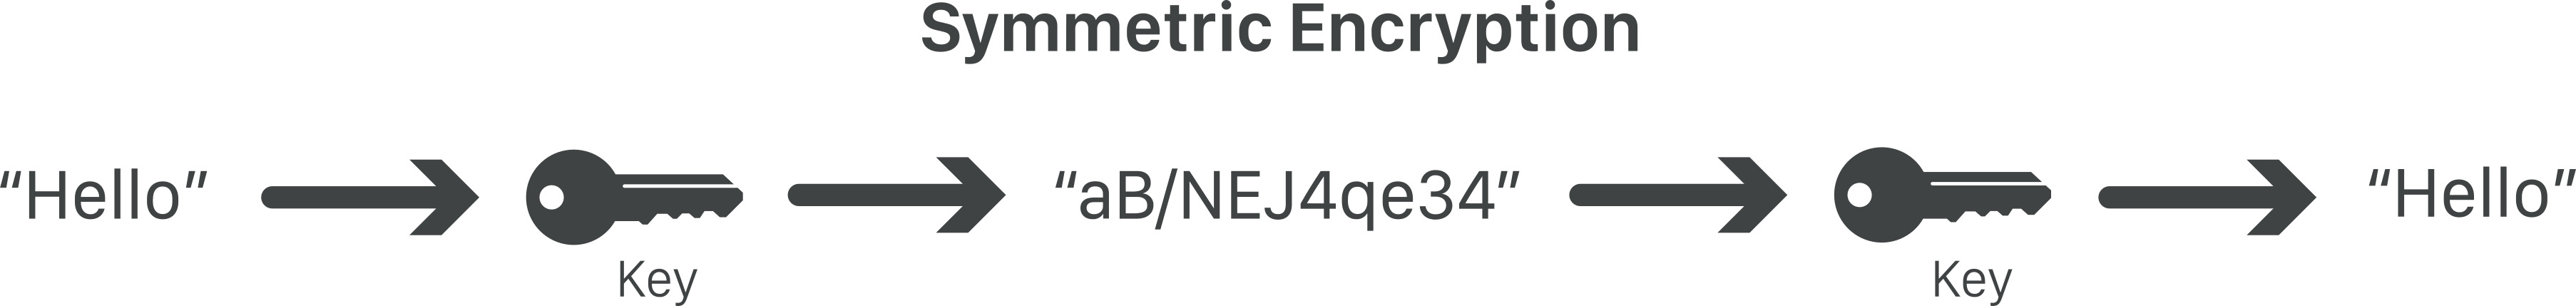
\includegraphics[width=0.8\textwidth]{\FIGURES/symmetric-encryption.jpg}
    \caption{Schéma symetrického šifrování. Zdroj: \parencite{cloudflare2024}}
    \label{fig:symmetric-encryption}
\end{figure}

Existují však i jiné způsoby relace, například v případě takzvaného \emph{session~resumption} (obnovení~relace). Tento mechanismus umožňuje serveru uchovávat šifrovací klíče po určitou dobu, čímž se eliminuje nutnost opětovného provádění celého TLS~handshake při každém novém spojení.

Podle dokumentace GnuTLS \textcite{gnutls2024}, existují dva hlavní způsoby obnovení relace:
\begin {enumerate}
\item \textit{Session~ID} - Server při prvním spojení klientovi přiřadí jedinečný identifikátor relace a dočasně uchová odpovídající šifrovací klíče. Při opětovném připojení klient odešle tento identifikátor a pokud server klíče stále uchovává, může relaci obnovit bez potřeby nového handshake.
\item \textit{Session~Tickets} - Místo aby server uchovával klíče, zašifruje je a pošle klientovi ve formě tzv. session ticketu. Při dalším spojení klient odešle ticket zpět serveru, který jej dešifruje a obnoví relaci. Tento přístup zlepšuje škálovatelnost, protože snižuje zátěž serveru spojenou s ukládáním velkého množství session~keys.
\end {enumerate}

Použití těchto metod nejen zvyšuje výkon a snižuje latenci při opakovaných připojeních, ale také umožňuje efektivnější správu šifrovacích operací, zejména u serverů s vysokým provozem. Nicméně, uchovávání klíčů delší dobu přináší i určitá bezpečnostní rizika - například pokud by došlo k úniku session keys, mohlo by to vést k dešifrování dříve zachycené komunikace (forward~secrecy).
Proto moderní verze TLS~, jako TLS~1.3, preferují ephemeral~key~exchange (pomíjivou výměnu klíčů), kde jsou klíče generovány pro každou relaci zvlášť a historii komunikace již tak nelze zpětně získat \parencite{gnutls2024}. 

Druhým příkladem hybridního šifrovacího systému je technologie~S/MIME, která se využívá pro zabezpečení e-mailové komunikace. Při použití S/MIME odesílatel nejprve digitálně podepíše email svým soukromým klíčem, čímž zajistí, že příjemce může ověřit autenticitu zprávy pomocí veřejného klíče odesílatele. Současně se pro samotné šifrování obsahu zprávy využívá symetrický klíč, který je následně bezpečně předán příjemci za použití asymetrického šifrovacího algoritmu. Tímto způsobem se spojují výhody asymetrické kryptografie a efektivity symetrického šifrování.
Výsledkem je systém, který nejen-že chrání důvěrnost odeslaných zpráv, ale také zaručuje integritu a nepopiratelnost komunikace mezi odesílatelem a příjemcem. Tento přístup se osvědčuje zejména v korporátním prostředí a v aplikacích, kde je klíčová bezpečnost e-mailové komunikace \parencite{cloudflare2024}.

\newpage